% fig11_pr_roll.tex — PR roll: lines-added per merged PR, hexa-lang kernels vs demiurge domain.
% Compiled by the paper Makefile via `make figures` (pdflatex on the snippet).
%
% Data provenance (NO fabrication; commons @D g3) — Appendix K (app:pr-roll):
%   All values are gh-measured (gh pr view --json additions), verbatim from
%   companion/pr-roll.json. 14 merged PRs total.
%   hexa-lang kernel/audit PRs (blue):
%     #1014=36  #1015=59  #1018=55  #1094=16  #1107=9
%   demiurge domain PRs (green):
%     #157=205 #158=96 #159=85 #162=122 #164=103 #166=113 #167=200 #168=80 #169=414
%   The point is the size asymmetry: the hexa-lang KERNELS are tiny (9-59 lines,
%   the closed-form is a few formulas) while the demiurge DOMAIN PRs (records,
%   scaffold, ledger) carry the bulk — exactly the stdlib-thin / domain-records
%   split the architecture predicts.
%
% Manual single-shot compile (debug):
%   pdflatex -interaction=nonstopmode -halt-on-error fig11_pr_roll.tex
\documentclass[border=4pt]{standalone}
\usepackage{amsmath}
\usepackage{tikz}
\usepackage{pgfplots}
\pgfplotsset{compat=1.18}
\begin{document}
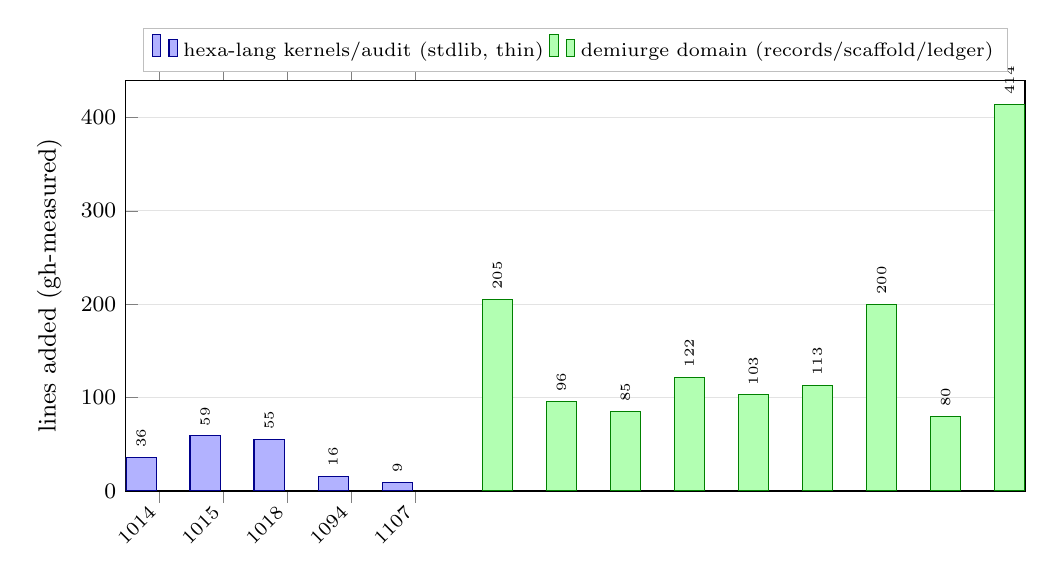
\begin{tikzpicture}
\begin{axis}[
  width=13cm, height=6.8cm,
  ybar,
  bar width=11pt,
  ymin=0, ymax=440,
  ylabel={lines added (gh-measured)},
  symbolic x coords={1014,1015,1018,1094,1107,157,158,159,162,164,166,167,168,169},
  xtick=data,
  x tick label style={font=\scriptsize,rotate=45,anchor=east},
  tick label style={font=\footnotesize},
  label style={font=\small},
  nodes near coords,
  nodes near coords style={font=\tiny,rotate=90,anchor=west},
  ymajorgrids, grid style={gray!22},
  enlarge x limits=0.04,
  legend style={font=\scriptsize, at={(0.5,1.02)}, anchor=south, legend columns=2,
    fill=white, draw=gray!50},
]
% hexa-lang kernel/audit PRs (blue)
\addplot[draw=blue!55!black, fill=blue!30] coordinates {
  (1014,36) (1015,59) (1018,55) (1094,16) (1107,9)
};
\addlegendentry{hexa-lang kernels/audit (stdlib, thin)}
% demiurge domain PRs (green)
\addplot[draw=green!50!black, fill=green!30] coordinates {
  (157,205) (158,96) (159,85) (162,122) (164,103) (166,113) (167,200) (168,80) (169,414)
};
\addlegendentry{demiurge domain (records/scaffold/ledger)}
\end{axis}
\end{tikzpicture}
\end{document}
